\documentclass{article}
\usepackage{graphicx} % Required for inserting images
\usepackage{float}
\usepackage[T1]{fontenc}
\usepackage{amsmath}
\usepackage[margin=1in]{geometry}
\usepackage{booktabs}
\usepackage{tabularx}
\usepackage[hidelinks]{hyperref}

\title{Tilting the put book's size toward steep-contango days cuts its risk but loses P\&L}
\author{Experiment report \textperiodcentered{} L/S Gamma Desk, QUANTT}
\date{2026-11-02}

\begin{document}

\maketitle

\textbf{Question:} On the 35\% stress-sized \texttt{hedged} put book, does scaling each entry's stress budget by the VIX term structure earn more net P\&L than the fixed 35\% budget, at 1x and 2x spreads, over the full window and in each half, without a worse tail or a drawdown beyond the budget? The scale runs from 1.5x in the steepest contango (VIX/\allowbreak{}VIX3M at its one-year low) to 0.5x at the most inverted (its one-year high).

\textbf{Method:}

\begin{itemize}

\item \textbf{Pre-registered backtest.} The research switches were committed in 73e16a4 and the hypothesis card in c74f769, before any run.

\item \textbf{Data and window.} The live paper rules (\texttt{configs/\allowbreak{}paper.\allowbreak{}toml}) are replayed on R2 replay snapshots v1 (config\_hash b040760187f0) over the development window 2014-06-02 to 2024-12-31. The hold-out (2025-01-01 to 2026-07-10) was not used.

\item \textbf{Book (all variants and the reference):} the \texttt{hedged} book of \texttt{2026-\allowbreak{}10-\allowbreak{}22-\allowbreak{}stress-\allowbreak{}sized-\allowbreak{}puts}.

\begin{itemize}

\item An always-on short 25-delta put, with the VRP signal ignored and the flat exit off.

\item Sized at entry so a one-day 20\% SPY drop, with IV at max(60\%, the put's IV), costs at most 35\% of \$250k.

\item Hedged daily at 10:15 with a 10-share band. The 1x-credit stop, 50\% profit-take, 7-DTE time exit and 1-day cool-off are as live.

\end{itemize}

\item \textbf{New switches.} \texttt{size\_\allowbreak{}by = ``vix\_\allowbreak{}vix3m''} and \texttt{size\_\allowbreak{}tilt} multiply the stress budget by 1 + tilt \ensuremath{\times} (2p \ensuremath{-} 1).

\begin{itemize}

\item p is the percentile of the prior close of VIX/\allowbreak{}VIX3M among its last 252 completed closes.

\item VIX/\allowbreak{}VIX3M below 1 is contango; above 1 is inverted.

\end{itemize}

\item \textbf{Variants:}

\begin{itemize}

\item \texttt{slope} (primary): tilt \ensuremath{-}0.5, so 1.5x at the one-year low of VIX/\allowbreak{}VIX3M and 0.5x at its high.

\item \texttt{slope\_\allowbreak{}light}: tilt \ensuremath{-}0.25 (0.75x to 1.25x).

\item \texttt{slope\_\allowbreak{}reverse}: tilt +0.5, larger when the curve is flat or inverted.

\end{itemize}

\item \textbf{Comparison:} the registered \texttt{2026-\allowbreak{}10-\allowbreak{}22-\allowbreak{}stress-\allowbreak{}sized-\allowbreak{}puts/\allowbreak{}hedged} runs, reused and not rerun, at the same spread multiple.

\item \textbf{Runs and costs:} every variant at 1x and 2x spreads. \$0.65 per contract and \$0.005 per share, with a \$1 minimum per order. Decisions, exits and hedges run once a day at 10:15 ET.

\end{itemize}

\section{Result vs the pass bar}

Every check had to hold at 1x and 2x spreads. P\&L, drawdown and ES are in USD on \$250k of capital. ES is the mean of the worst 5\% of daily P\&L.

\begin{center}\small
\begin{tabularx}{\linewidth}{>{\raggedright\arraybackslash}X l l l l l}
\toprule
\textbf{Check (\texttt{slope} vs \texttt{hedged})} & \textbf{1x value} & \textbf{1x bar} & \textbf{2x value} & \textbf{2x bar} & \textbf{Result} \\
\midrule
Net P\&L, full window & \$100,574 & > \$121,482 & \$78,318 & > \$101,172 & fail \\
Net P\&L, 2014-06 to 2019-12 & \$43,556 & > \$49,132 & \$34,608 & > \$42,687 & fail \\
Net P\&L, 2020-01 to 2024-12 & \$57,018 & > \$72,350 & \$43,710 & > \$58,485 & fail \\
ES 5\% within 1.10x & \ensuremath{-}\$2,471 & \ensuremath{\geq} \ensuremath{-}\$3,317 & \ensuremath{-}\$2,565 & \ensuremath{\geq} \ensuremath{-}\$3,404 & pass \\
Max drawdown within the budget & \$42,017 & \ensuremath{\leq} \$87,500 & \$46,035 & \ensuremath{\leq} \$87,500 & pass \\
Round trips (floor 30) & 182 & \ensuremath{\geq} 30 &  &  & met \\
\bottomrule
\end{tabularx}
\end{center}

\textbf{Verdict: failed.} The term-structure tilt made the book safer but not more profitable. Net P\&L fell by \$20.9k at 1x and \$22.9k at 2x, and it fell in both halves. Drawdown fell from \$70k to \$42k at 1x, and Sharpe rose from 0.52 to 0.64. The book still makes money: about \$100k at 1x and \$78k at 2x over 10.6 years.

\subsection{Full-window numbers (not part of the bar)}

\textbf{1x spreads}

\begin{center}\small
\begin{tabularx}{\linewidth}{>{\raggedright\arraybackslash}X >{\raggedright\arraybackslash}X >{\raggedright\arraybackslash}X >{\raggedright\arraybackslash}X >{\raggedright\arraybackslash}X}
\toprule
\textbf{} & \textbf{hedged} & \textbf{slope} & \textbf{slope\_light} & \textbf{slope\_reverse} \\
\midrule
Net P\&L & \$121,482 & \$100,574 & \$110,707 & \$121,007 \\
Sharpe & 0.52 & 0.64 & 0.58 & 0.45 \\
Max drawdown & \$70,362 & \$42,017 & \$56,030 & \$53,207 \\
ES 5\% (daily) & \ensuremath{-}\$3,016 & \ensuremath{-}\$2,471 & \ensuremath{-}\$2,728 & \ensuremath{-}\$3,456 \\
Round trips & 182 & 182 & 183 & 181 \\
Contracts per entry, mean /\allowbreak{} max & 25.4 /\allowbreak{} 100 & 24.7 /\allowbreak{} 52 & 25.0 /\allowbreak{} 75 & 25.7 /\allowbreak{} 131 \\
Commissions, options /\allowbreak{} hedges & \$5,955 /\allowbreak{} \$2,868 & \$5,810 /\allowbreak{} \$2,882 & \$5,916 /\allowbreak{} \$2,864 & \$5,996 /\allowbreak{} \$2,893 \\
\bottomrule
\end{tabularx}
\end{center}

\textbf{2x spreads}

\begin{center}\small
\begin{tabularx}{\linewidth}{>{\raggedright\arraybackslash}X l l l >{\raggedright\arraybackslash}X}
\toprule
\textbf{} & \textbf{hedged} & \textbf{slope} & \textbf{slope\_light} & \textbf{slope\_reverse} \\
\midrule
Net P\&L & \$101,172 & \$78,318 & \$88,923 & \$119,011 \\
Sharpe & 0.43 & 0.49 & 0.46 & 0.39 \\
Max drawdown & \$75,488 & \$46,035 & \$60,583 & \$84,190 \\
ES 5\% (daily) & \ensuremath{-}\$3,094 & \ensuremath{-}\$2,565 & \ensuremath{-}\$2,809 & \ensuremath{-}\$3,505 \\
\bottomrule
\end{tabularx}
\end{center}

\section{Charts}

\begin{figure}[H]\centering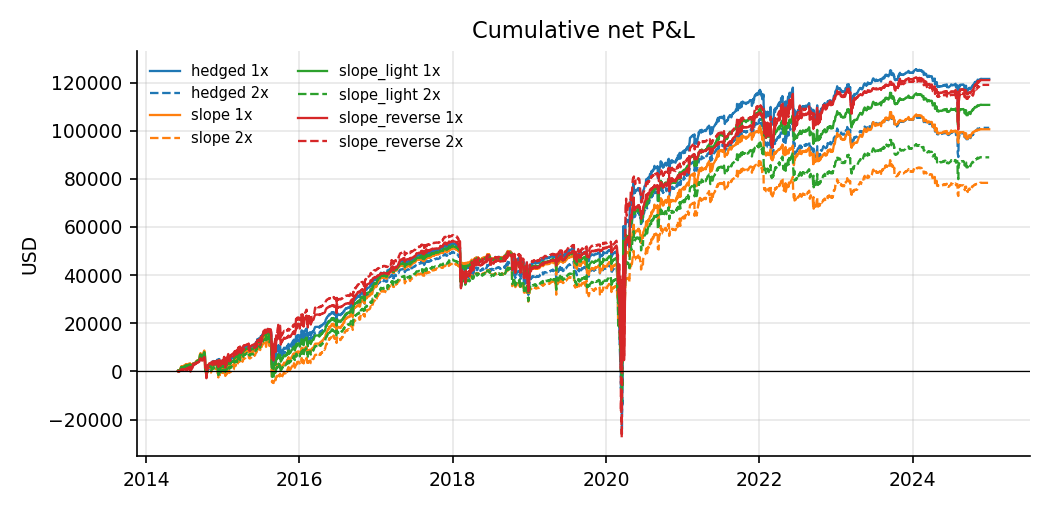
\includegraphics[width=0.92\linewidth]{figures/cum_pnl.png}\caption{Cumulative net P\&L, 1x solid and 2x dashed}\end{figure}

All four books follow the same path, because they hold the same put on most days: 173 of \texttt{slope}'s 182 entries fall on the same day as an entry of \texttt{hedged}. \texttt{slope} falls behind in 2014-2015 and in March 2020, and never catches up. \texttt{slope\_\allowbreak{}reverse} ends level with \texttt{hedged} at 1x and ahead at 2x.

\begin{figure}[H]\centering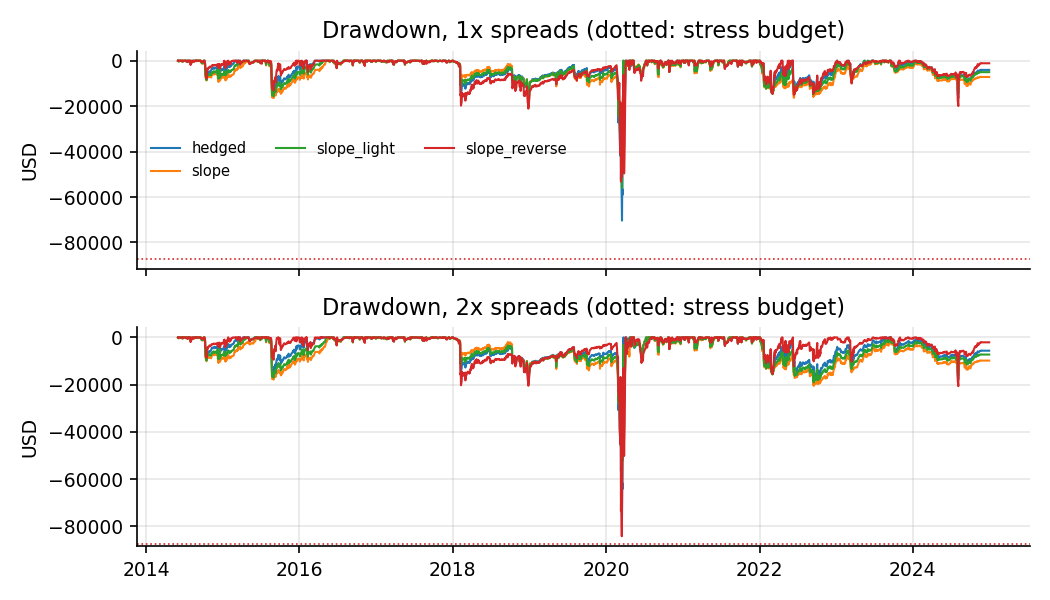
\includegraphics[width=0.92\linewidth]{figures/drawdown.png}\caption{Drawdown at 1x and 2x spreads; dotted line: the \$87,500 stress budget}\end{figure}

The deepest drawdown of \texttt{hedged}, \texttt{slope} and \texttt{slope\_\allowbreak{}light} falls on 17 March 2020 (\texttt{slope\_\allowbreak{}reverse}: 12 March at 1x, 16 March at 2x). \texttt{slope} loses \$42k there against \texttt{hedged}'s \$70k, because it entered the spike at half size. \texttt{slope\_\allowbreak{}reverse} comes within \$3.3k of the budget at 2x (\$84.2k).

\begin{figure}[H]\centering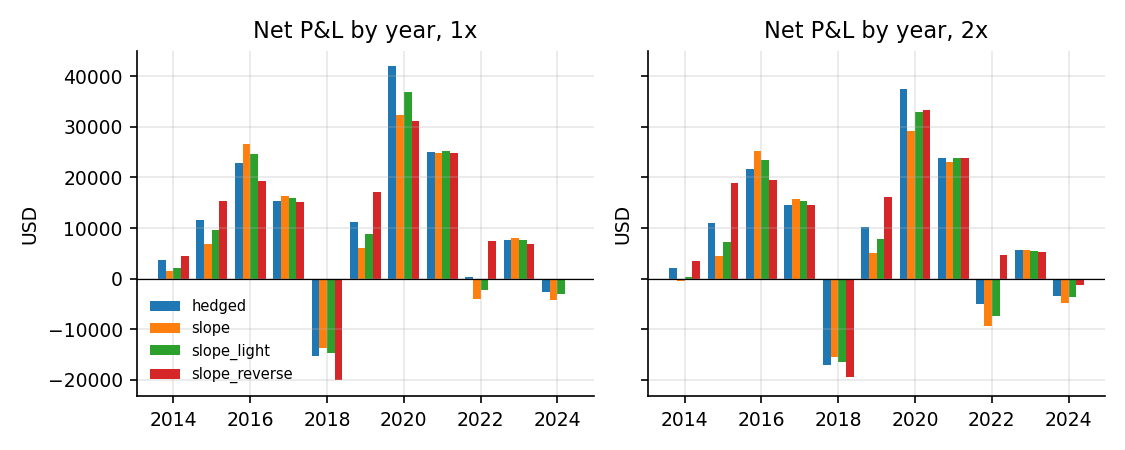
\includegraphics[width=0.92\linewidth]{figures/yearly.png}\caption{Net P\&L by year}\end{figure}

\texttt{slope} makes less than \texttt{hedged} in 7 of 11 years at 1x. The largest gaps are 2020 (\ensuremath{-}\$9.7k), 2019 (\ensuremath{-}\$5.1k), 2015 (\ensuremath{-}\$4.7k) and 2022 (\ensuremath{-}\$4.4k). It makes more only in 2016, 2017, 2018 and 2023, by \$0.4k to \$3.8k each.

\begin{figure}[H]\centering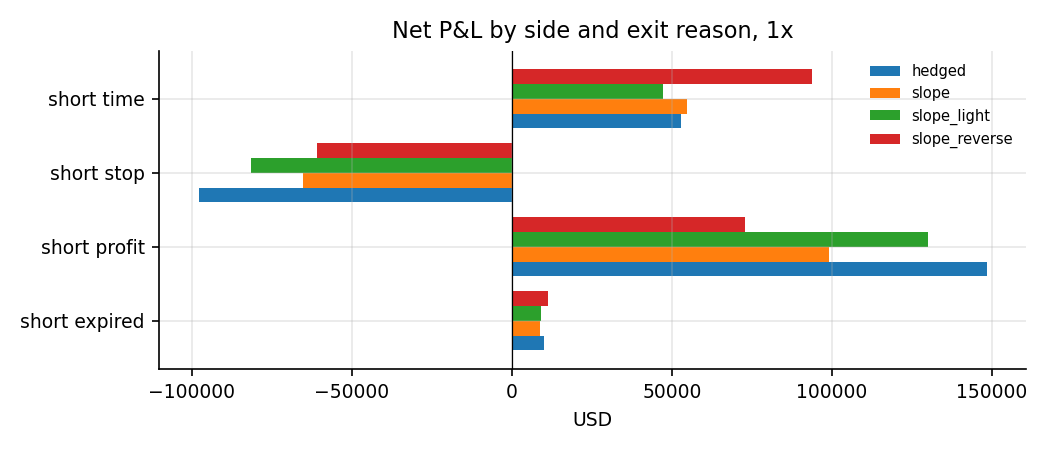
\includegraphics[width=0.92\linewidth]{figures/by_reason.png}\caption{Net P\&L by side and exit reason, 1x}\end{figure}

\texttt{slope} cuts stop losses by about a third against \texttt{hedged}, but its profit-takes shrink more. It sold less on the stressed days whose puts later paid off.

\begin{figure}[H]\centering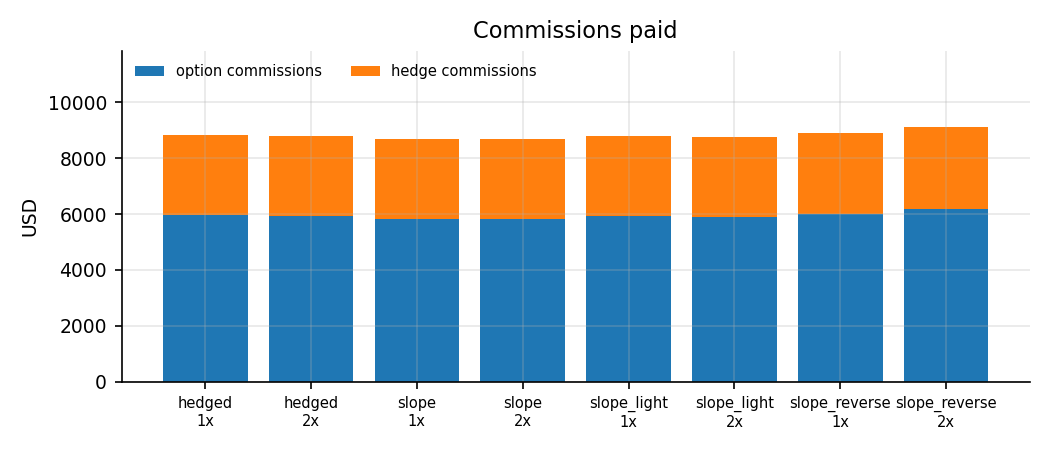
\includegraphics[width=0.92\linewidth]{figures/fees.png}\caption{Commissions paid}\end{figure}

Commissions barely move (\$8.7k to \$9.1k across all books), because average size is almost unchanged. Costs don't explain the result.

\begin{figure}[H]\centering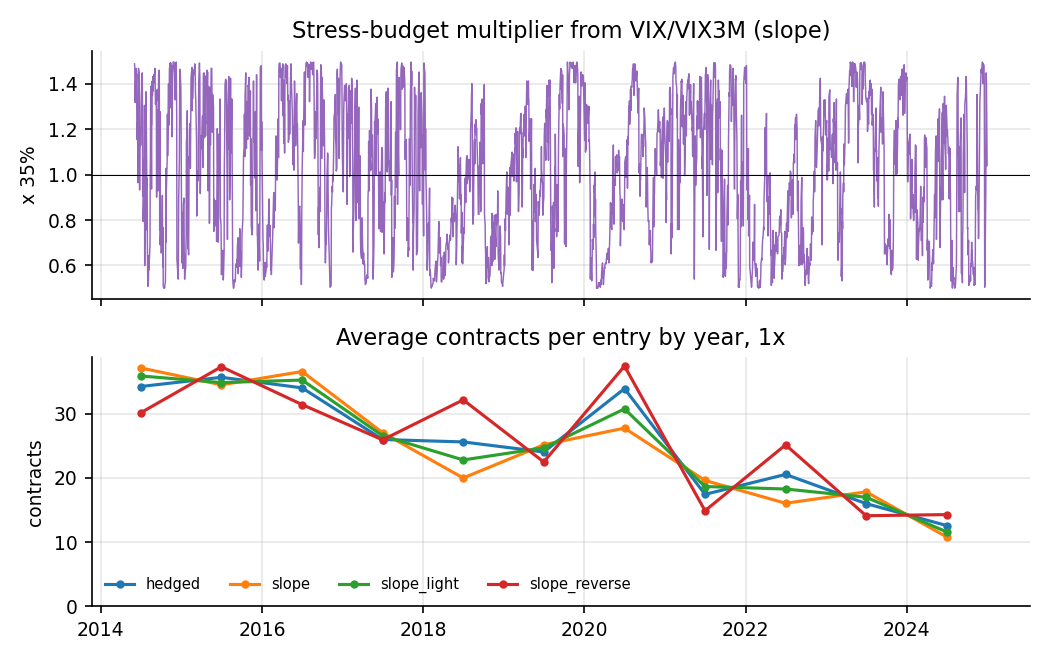
\includegraphics[width=0.92\linewidth]{figures/multiplier.png}\caption{Stress-budget multiplier from VIX/\allowbreak{}VIX3M (top) and average contracts per entry by year (bottom)}\end{figure}

The multiplier swings between 0.5x and 1.5x within weeks, and its daily mean over the window is 1.02. Average contracts per entry stay close to \texttt{hedged} in most years. The largest gaps are in 2018, 2020 and 2022, years with curve inversions, when \texttt{slope} sold less.

\section{Analysis}

\textbf{The tilt removed the book's biggest winners.} In early 2020 VIX/\allowbreak{}VIX3M was at or near its one-year high. The book made five entries between 26 February and 17 April 2020, all on the same days in \texttt{slope} and \texttt{hedged}. Three were sized at the 0.5x floor, and the others at 0.57x and 0.67x.

\begin{itemize}

\item The two large entries were cut from 100 and 71 contracts to 50 and 40.

\item Those five round trips made \$14.3k for \texttt{slope} against \$22.9k for \texttt{hedged}.

\item That is mechanical. Cutting size into the vol spike cuts both the drawdown on 17 March and the recovery that followed by about 40\%.

\end{itemize}

The same happened in smaller spikes: \texttt{slope} gave up \$4.7k in 2015, \$5.1k in 2019 and \$4.4k in 2022. The two largest round trips made 72\% of \texttt{hedged}'s round-trip net, but only 44\% of \texttt{slope}'s. The concentration flagged in the 2026-10-22 report is much smaller here, but the P\&L went with it.

\textbf{The signal doesn't sort per-contract P\&L.} In the reference \texttt{hedged} book, net P\&L per contract by multiplier tercile at entry was:

\begin{center}\small
\begin{tabularx}{\linewidth}{>{\raggedright\arraybackslash}X l >{\raggedright\arraybackslash}X l >{\raggedright\arraybackslash}X}
\toprule
\textbf{Tercile at entry} & \textbf{Round trips} & \textbf{Mean multiplier} & \textbf{Per contract} & \textbf{Standard error} \\
\midrule
Low (curve flattest or inverted) & 62 & 0.65 & \$6.1 & \$32.5 \\
Middle & 59 & 1.01 & \$0.4 & \$16.7 \\
High (steepest contango) & 61 & 1.36 & \$24.3 & \$13.9 \\
\bottomrule
\end{tabularx}
\end{center}

\begin{itemize}

\item The rank correlation between the multiplier and per-contract P\&L is \ensuremath{-}0.004.

\item The high tercile looks better, but the gaps are within one or two standard errors. Per-contract numbers are equal-weighted, while the low tercile's dollar P\&L (\$62.8k, the largest) comes from a few large, high-IV entries.

\item So the tilt moves size from where the dollars were made to where they weren't. That is the opposite of what the hypothesis needs. Johnson's (2017) evidence is for variance swaps, VIX futures and straddles, not a 25-delta put held to 7 DTE.

\end{itemize}

\textbf{The reverse tilt is not a fix.} \texttt{slope\_\allowbreak{}reverse} sold 131 contracts at one 2020 entry. It matched \texttt{hedged}'s P\&L at 1x (\$121.0k) and beat it at 2x (\$119.0k), but with a lower Sharpe (0.45 /\allowbreak{} 0.39) and a worse tail. Its 2x drawdown of \$84.2k nearly used the whole budget.

\begin{itemize}

\item It is a sensitivity, so it can't pass this card.

\item Its entry path in 2020 differs from the others (its entry dates diverge from the other books from late 2019, and it held through March on time exits), so its 2020 result is partly path, not signal.

\item Its 2x lead comes mostly from 2015, 2019 and 2022, the same years where \texttt{slope} lost.

\end{itemize}

\texttt{slope\_\allowbreak{}light} sits between \texttt{hedged} and \texttt{slope} on every headline metric: half the tilt gives about half the P\&L loss and half the drawdown cut. That's what a mechanical size effect looks like, not a timing effect.

\section{Verdict}

\textbf{Failed.} The book's P\&L fell at both spreads and in both halves; the tail and drawdown checks passed. Archive the term-structure tilt as a profit signal.

What it did do is cut risk: Sharpe 0.64 against 0.52 at 1x, and drawdown \$42k against \$70k. That is roughly what a lower fixed budget would do. A follow-up that compares this tilt with a plain fixed budget of the same average risk would need its own card. The 15\% and 25\% budgets the PM asked for on 2026-10-22 cover most of that question.

\section{Caveats}

\begin{itemize}

\item \textbf{In-sample:}

\begin{itemize}

\item The idea came from the 2026-10-31 strategy research report (literature).

\item The book is the 2026-10-22 primary, chosen after its results.

\item The desk's earlier gate tests had already shown that skipping shorts on an inverted curve removed profit.

\end{itemize}

\item \textbf{One big episode:} much of the gap comes from March 2020. One crash dominates the comparison, so the size of the effect is uncertain. The direction is consistent across 7 of 11 years.

\item \textbf{Sizing input:} the percentile is of VIX/\allowbreak{}VIX3M's prior close among the last 252 completed closes. VIX3M (with VVIX and VIX9D) comes from a frozen yfinance download.

\item \textbf{Stress model:} Black-Scholes, an instantaneous 20\% drop and no vol shock above 60\% IV. The tilt scales the budget, not the scenario.

\item \textbf{Spread model:} fitted on about two weeks of calm 2026 live quotes; the 2x run is the stress test. Fills of 50-131 contracts use the same model as one contract.

\item \textbf{Margin:} not modelled.

\item \textbf{Data gaps:} about 3.3\% of scheduled times are skipped (89 days, the same in every run). Every run had 9 unfilled orders at 1x.

\end{itemize}

\section{Trials}

6 trials for this experiment (3 variants \ensuremath{\times} 1x and 2x, one run of \texttt{experiment.\allowbreak{}py}), plus the baseline's 2. The runs are tagged with the branch head, 954824c, which adds only another card's pre-registration after c74f769. The two \texttt{slope\_\allowbreak{}reverse} rows are tagged \texttt{-\allowbreak{}dirty}: during the run, a parallel experiment's reporting script was edited in the working tree. The engine, configs and this card's files were unchanged from 954824c. The \texttt{hedged} reference was reused from \texttt{2026-\allowbreak{}10-\allowbreak{}22-\allowbreak{}stress-\allowbreak{}sized-\allowbreak{}puts} (2 trials, not rerun). The registry holds 98 trials in all, after the four 2026-11-02 cards. The pass bar was not changed.

\end{document}
